\section{Method}
\label{sec:method}

KG-SCoRE takes a biomedical KG derived from SemMedDB-style triples and a research question, and outputs ranked, traceable hypotheses. Figure~\ref{fig:framework} shows the four modules. We detail each below.

\begin{figure}[tb]
  \centering
  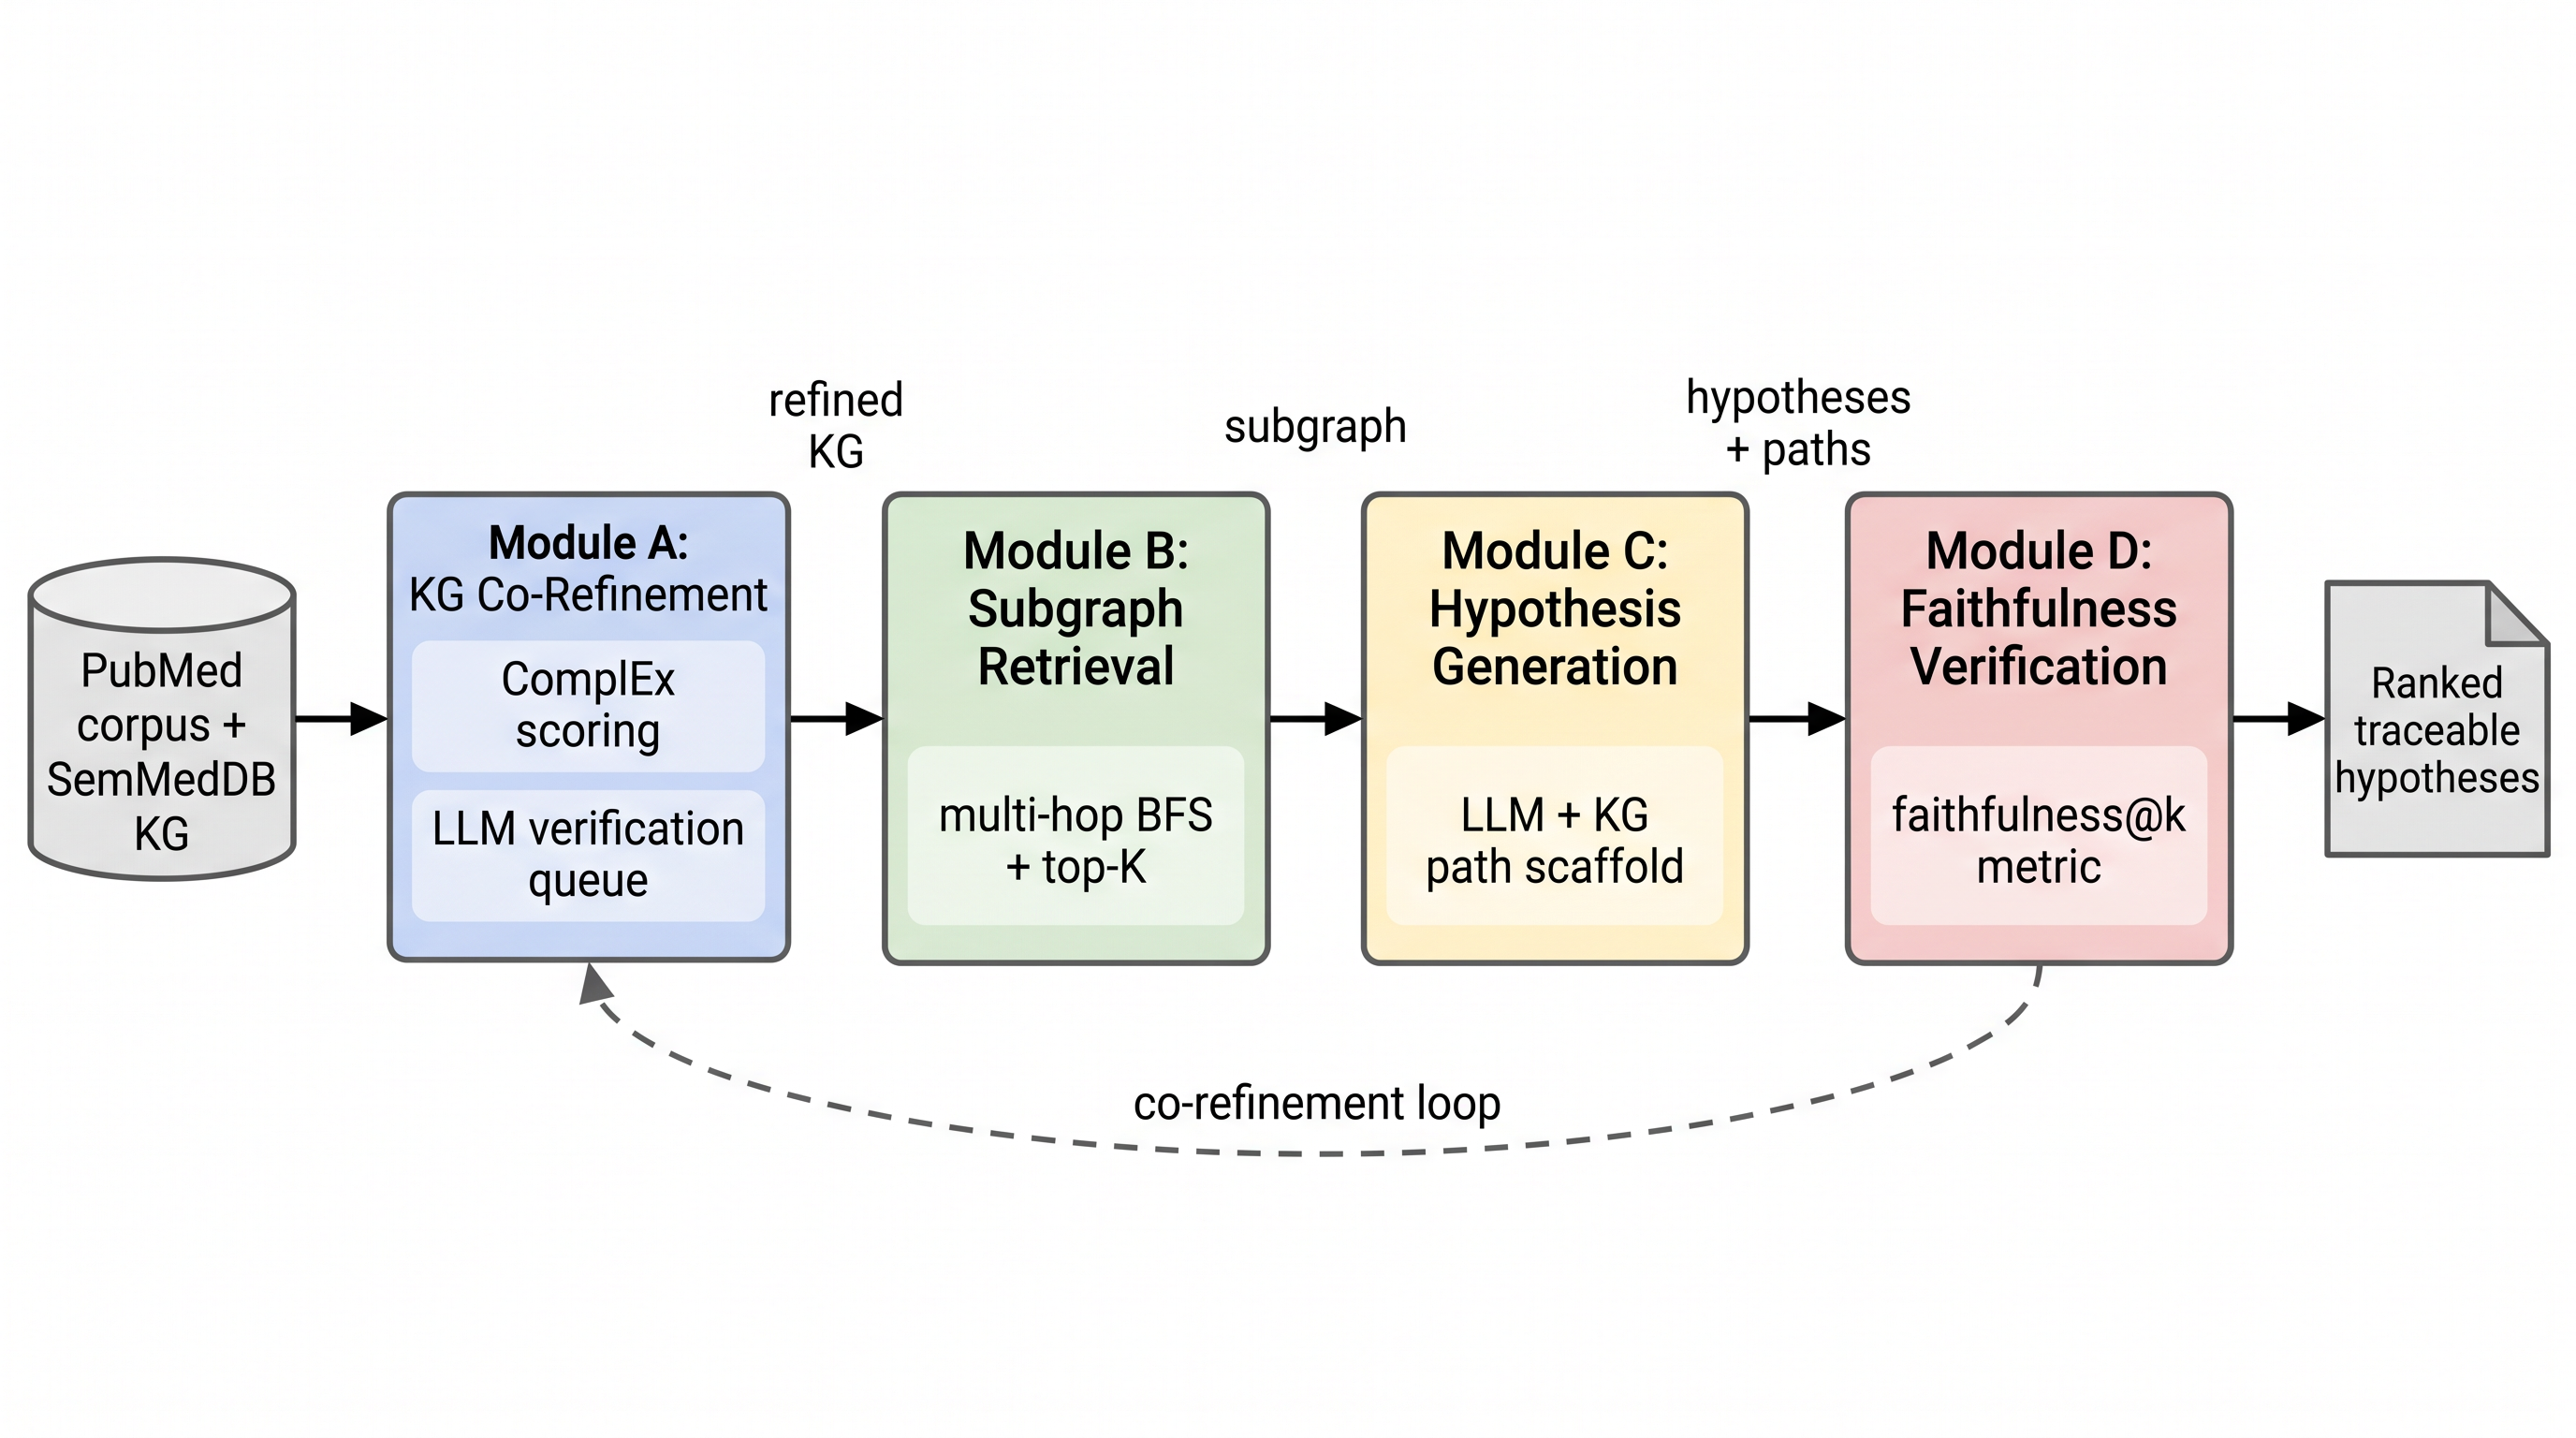
\includegraphics[width=\linewidth]{figures/framework.png}
  \caption{KG-SCoRE pipeline. Module~A verifies KG triples via LLM prompting (optionally gated by ComplEx scores). Module~B retrieves scored multi-hop subgraphs. Module~C generates KG-scaffolded hypotheses. Module~D verifies faithfulness against KG paths.}
  \label{fig:framework}
\end{figure}

\subsection{Problem Formulation}
Let $\mathcal{G}=(\mathcal{E},\mathcal{R},\mathcal{T})$ be a KG with entities $\mathcal{E}$, relations $\mathcal{R}$, and triples $\mathcal{T}=\{(h,r,t)\}$. Given a research question $q$ with seed entity $e_s\in\mathcal{E}$, the goal is to produce a ranked list of hypotheses $\mathcal{H}=\{h_1,\dots,h_K\}$, where each $h_i$ is associated with a KG path $\pi_i=(e_s,r_1,e_1,\dots,r_m,e_t)$, such that (i) $h_i$ is \emph{novel}: the direct link $e_s\!\to\!e_t$ is not stated in $\mathcal{T}$ (though a multi-hop path $e_s \xrightarrow{r_1} \cdots \xrightarrow{r_m} e_t$ may exist), and (ii) $h_i$ is \emph{faithful}: it is entailed by $\pi_i$.

\subsection{Module A: KG Verification}
\label{sec:method:a}

Module~A cleans and audits the KG by verifying triples via LLM prompting. An optional ComplEx-based scoring stage can gate which triples are verified.

\paragraph{Optional learned triple scoring.}
We may train a ComplEx~\cite{trouillon2016complex} embedding model on $\mathcal{T}$. Each entity $e$ and relation $r$ is mapped to complex vectors $\mathbf{e},\mathbf{r}\in\mathbb{C}^d$. The plausibility of a triple $(h,r,t)$ is
\begin{equation}
  \label{eq:complex}
  s(h,r,t) = \mathrm{Re}\!\left(\sum_{k=1}^{d} \mathbf{h}_k\,\mathbf{r}_k\,\overline{\mathbf{t}_k}\right),
\end{equation}
trained with negative sampling and softplus loss. After training, every triple receives a score $s_i$; low scores flag potentially noisy triples. However, as our experiments show (Sec.~\ref{sec:exp:ablation}), when the KG-completion model has low MRR, this gating is counterproductive. In the primary configuration, \textbf{all} retrieved triples are verified by the LLM without ComplEx gating.

\paragraph{LLM verification.}
For each triple in the \emph{query-local} retrieved subgraph $\mathcal{S}(e_s)$ (not the global KG), we prompt the LLM with the triple and optional text context, asking it to output a verdict $v\in\{\textsc{supported},\textsc{contradicted},\textsc{unverifiable}\}$ and, if contradicted, a corrected object $\hat{t}$. The verified subgraph $\mathcal{S}'$ is:
\begin{equation}
  \mathcal{S}' = \{(h,r,t)\in\mathcal{S}\mid v=\textsc{supported}\}\;\cup\;\{(h,r,\hat{t})\mid v=\textsc{contradicted}\}\;\cup\;\mathcal{U},
\end{equation}
where $\mathcal{U}$ is the set of \textsc{unverifiable} triples. In the primary (conservative) mode, $\mathcal{U}$ is retained (only \textsc{contradicted}-without-correction triples are deleted), avoiding over-deletion; in the aggressive mode, $\mathcal{U}=\emptyset$. Verification is performed per query on the retrieved subgraph; corrections are not written back to the global KG, so this is a \emph{query-time} verification rather than a global KG rewrite. This distinction is reflected in our naming: \emph{query-time KG verification} rather than global co-refinement.

\paragraph{Prompt design.}
The verification prompt provides the triple $(h, r, t)$ with the entity types of $h$ and $t$, and asks the LLM to (i) check type-relation validity, (ii) check direction (e.g., \texttt{TREATS} points chemical$\to$disease), and (iii) judge biomedical support, returning a structured JSON verdict. Prompt templates for all modules are in the released code.

\paragraph{Complexity.}
For each query, Module~A verifies $K{=}40$ retrieved triples ($K$ LLM calls). Module~C requires 1 LLM call to overgenerate $M{=}20$ candidate hypotheses. Module~D verifies each of the $M$ hypotheses for faithfulness ($M$ LLM calls). The total is $K{+}1{+}M = 40{+}1{+}20 = 61$ LLM calls per query. At GPT-4o-mini pricing (\$0.15/M input tokens, \$0.60/M output tokens), the average cost per query is approximately \$0.03, making the pipeline practical for batch hypothesis generation.

\subsection{Module B: Symbolic Subgraph Retrieval}
\label{sec:method:b}

Given seed entity $e_s$, we perform bounded-depth BFS over $\mathcal{G}'$ up to $L$ hops ($L{=}2$), collecting triples along the way. The subgraph $\mathcal{S}(e_s)$ is the top-$K$ triples:
\begin{equation}
  \mathcal{S}(e_s) = \mathrm{TopK}_{(h,r,t)\in\mathrm{BFS}_L(e_s;\,\mathcal{G}')}\; |s(h,r,t)|.
\end{equation}
In the primary configuration (no ComplEx), all retrieved triples are ranked by retrieval order.

\paragraph{Subgraph size and hop depth.}
We set $K{=}40$ and $L{=}2$ based on preliminary analysis: $K{=}40$ covers $\sim$85\% of the 2-hop neighborhood, and $L{=}2$ captures the classic LBD pattern (disease $\to$ intermediate $\to$ chemical). Larger $K$ or $L$ gave diminishing returns at higher cost.

\subsection{Module C: Symbolic-Scaffolded Generation}
\label{sec:method:c}

We prompt the LLM with the research question $q$, the subgraph $\mathcal{S}(e_s)$ rendered as pipe-delimited triples, and optional text snippets. The prompt instructs the LLM to (i) reason step-by-step over KG paths, (ii) generate $M$ ranked hypotheses, and (iii) for each hypothesis emit an explicit \texttt{KG\_PATH} chain $e_s\!\xrightarrow{r_1}\!e_1\!\xrightarrow{r_2}\!\cdots\!\xrightarrow{r_m}\!e_t$. Forcing the path output enables downstream faithfulness verification. The prompt also includes a novelty instruction: the LLM should prefer target entities $e_t$ that are \emph{not} directly linked to $e_s$ in $\mathcal{T}$, encouraging genuine discovery rather than restating known facts. We \emph{overgenerate} $M{=}20$ hypotheses so that faithfulness-guided reranking (Module~D) has candidates to promote, and return the top 10 after reranking to match the LBD Hit@10 protocol.

\subsection{Module D: Faithfulness Verification}
\label{sec:method:d}

For each hypothesis $h_i$ with path $\pi_i$, we prompt the LLM (as a strict judge) to classify entailment as $f_i\in\{\textsc{entailed},\textsc{partial},\textsc{none}\}$. We report two variants of the metric:
\begin{equation}
  \label{eq:faith_strict}
  \mathrm{StrictFaith}@k = \frac{1}{\min(k,|\mathcal{H}|)}\sum_{i=1}^{\min(k,|\mathcal{H}|)} \mathbb{1}\!\left[f_i=\textsc{entailed}\right],
\end{equation}
\begin{equation}
  \label{eq:faith_broad}
  \mathrm{BroadFaith}@k = \frac{1}{\min(k,|\mathcal{H}|)}\sum_{i=1}^{\min(k,|\mathcal{H}|)} \mathbb{1}\!\left[f_i\in\{\textsc{entailed},\textsc{partial}\}\right].
\end{equation}
StrictFaith counts only fully entailed hypotheses; BroadFaith also counts partial support. We additionally report \emph{path coverage}: the fraction of hypotheses for which a KG path can be extracted. This decomposition addresses the concern that counting ``partial'' as faithful may overstate grounding.

Unlike text-overlap faithfulness metrics used in RAG~\cite{brown2025systematic}, our metric verifies entailment against structured symbolic paths. While RoG~\cite{luo2024graphconstrained} constrains generation to KG-grounded paths during decoding, it does not post-hoc verify whether the final output is entailed by a specific path; KG-SCoRE adds both verification and \emph{faithfulness-guided reranking}.

\paragraph{Faithfulness-guided reranking.}
After Module~D labels each hypothesis, we \emph{rerank} the hypothesis list by faithfulness: \textsc{entailed} hypotheses are promoted to the top, followed by \textsc{partial}, then \textsc{none}. Within each tier, the original LLM ranking is preserved. To ensure sufficient candidates for reranking, we overgenerate $K{=}20$ hypotheses and return the top-10 after reranking. This is a key algorithmic contribution: Module~D does not merely \emph{measure} faithfulness---it actively \emph{shapes} the output by ensuring that the most traceable hypotheses appear first. For KGQA tasks, a separate prompt allows the LLM to leverage both the KG and parametric knowledge, while still applying faithfulness reranking.

\paragraph{Entailment classification criteria.}
The LLM judge applies three criteria: (1) \textsc{entailed} requires that every claim in $h_i$ is directly supported by $\pi_i$---no additional information is introduced; (2) \textsc{partial} requires that the core claim (the source--target link) follows from $\pi_i$, but the hypothesis may add explanatory mechanisms, causal claims, or quantitative details not present in the path; (3) \textsc{none} means the hypothesis contradicts $\pi_i$ or introduces a claim with no path support. This three-level scheme captures a meaningful distinction: \textsc{entailed} hypotheses are fully auditable, while \textsc{partial} hypotheses require human review of the additional claims. As our experiments show (Sec.~\ref{sec:exp:faith}), the boundary between \textsc{entailed} and \textsc{partial} is sensitive to judge design ($\kappa{\approx}0$), motivating the dual-metric reporting.

\paragraph{Formal novelty definition.}
A hypothesis $h_i$ with target entity $e_t$ is \emph{novel} if the direct triple $(e_s, r^*, e_t) \notin \mathcal{T}$ for any relation $r^* \in \mathcal{R}$. That is, the gold answer is not directly stated in the KG, though a multi-hop path $e_s \xrightarrow{r_1} \cdots \xrightarrow{r_m} e_t$ may exist. This definition aligns with the LBD task: the goal is to discover connections not explicitly recorded, even if indirect evidence chains exist. In practice, we enforce novelty by filtering out hypotheses whose target entity has a direct edge from $e_s$ in $\mathcal{T}$.

\subsection{Full Pipeline and Ablation Configurations}
Algorithm~\ref{alg:kgscore} summarizes the pipeline. ComplEx scoring (Line 1) is \emph{optional}; the primary configuration skips it and verifies all retrieved triples. Ablation configurations: \texttt{raw\_kg} (no verification), \texttt{+llm} (LLM verification, no faithfulness check), \texttt{+llm+faith} (LLM verification + faithfulness, no ComplEx — the primary mode), \texttt{+learned} (ComplEx scoring only), \texttt{full} (all modules including ComplEx), \texttt{no\_kg} (KG scaffold off), \texttt{no\_faith} (Module~D off).

\begin{algorithm}[tb]
\caption{KG-SCoRE inference}
\label{alg:kgscore}
\begin{algorithmic}[1]
\Require KG $\mathcal{G}$, question $q$, seed $e_s$, params $K,L,M$
\Statex \textcolor{gray}{\textit{// Optional: ComplEx scoring (Module A)}}
\If{ComplEx enabled}
  \State Train ComplEx on $\mathcal{T}$; compute scores $s_i$
  \State $\mathcal{G}' \gets \mathrm{Filter}(\mathcal{G}, \{s_i\}, \tau)$
\Else
  \State $\mathcal{G}' \gets \mathcal{G}$
\EndIf
\State $\mathcal{S} \gets \mathrm{TopK}_K(\mathrm{BFS}_L(e_s;\, \mathcal{G}'))$ \Comment{Module B}
\State $\mathcal{S}' \gets \mathrm{LLM\_Verify}(\mathcal{S})$ \Comment{Module A: clean subgraph}
\State $\mathcal{H} \gets \mathrm{LLM\_Generate}(q, \mathcal{S}',\, M)$ with paths $\{\pi_i\}$ \Comment{Module C}
\State $f_i \gets \mathrm{LLM\_Judge}(h_i, \pi_i)$ for each $h_i \in \mathcal{H}$ \Comment{Module D}
\State $\mathcal{H} \gets \mathrm{RerankByFaithfulness}(\mathcal{H}, \{f_i\})$ \Comment{entailed $>$ partial $>$ none}
\State \Return top-10 of $\mathcal{H}$ with faithfulness labels
\end{algorithmic}
\end{algorithm}
